% Options for packages loaded elsewhere
\PassOptionsToPackage{unicode}{hyperref}
\PassOptionsToPackage{hyphens}{url}
%
\documentclass[
  12pt,a4paper,lualatex,ja=standard]{bxjsarticle}
\usepackage{lmodern}
\usepackage{amsmath}
\usepackage{ifxetex,ifluatex}
\ifnum 0\ifxetex 1\fi\ifluatex 1\fi=0 % if pdftex
  \usepackage[T1]{fontenc}
  \usepackage[utf8]{inputenc}
  \usepackage{textcomp} % provide euro and other symbols
  \usepackage{amssymb}
\else % if luatex or xetex
  \usepackage{unicode-math}
  \defaultfontfeatures{Scale=MatchLowercase}
  \defaultfontfeatures[\rmfamily]{Ligatures=TeX,Scale=1}
\fi
% Use upquote if available, for straight quotes in verbatim environments
\IfFileExists{upquote.sty}{\usepackage{upquote}}{}
\IfFileExists{microtype.sty}{% use microtype if available
  \usepackage[]{microtype}
  \UseMicrotypeSet[protrusion]{basicmath} % disable protrusion for tt fonts
}{}
\makeatletter
\@ifundefined{KOMAClassName}{% if non-KOMA class
  \IfFileExists{parskip.sty}{%
    \usepackage{parskip}
  }{% else
    \setlength{\parindent}{0pt}
    \setlength{\parskip}{6pt plus 2pt minus 1pt}}
}{% if KOMA class
  \KOMAoptions{parskip=half}}
\makeatother
\usepackage{xcolor}
\IfFileExists{xurl.sty}{\usepackage{xurl}}{} % add URL line breaks if available
\IfFileExists{bookmark.sty}{\usepackage{bookmark}}{\usepackage{hyperref}}
\hypersetup{
  hidelinks,
  pdfcreator={LaTeX via pandoc}}
\urlstyle{same} % disable monospaced font for URLs
\usepackage{graphicx}
\makeatletter
\def\maxwidth{\ifdim\Gin@nat@width>\linewidth\linewidth\else\Gin@nat@width\fi}
\def\maxheight{\ifdim\Gin@nat@height>\textheight\textheight\else\Gin@nat@height\fi}
\makeatother
% Scale images if necessary, so that they will not overflow the page
% margins by default, and it is still possible to overwrite the defaults
% using explicit options in \includegraphics[width, height, ...]{}
\setkeys{Gin}{width=\maxwidth,height=\maxheight,keepaspectratio}
% Set default figure placement to htbp
\makeatletter
\def\fps@figure{htbp}
\makeatother
\setlength{\emergencystretch}{3em} % prevent overfull lines
\providecommand{\tightlist}{%
  \setlength{\itemsep}{0pt}\setlength{\parskip}{0pt}}
\setcounter{secnumdepth}{5}
\usepackage{indentfirst}
\parindent = 1em
\usepackage{dcolumn}
\newcolumntype{.}{D{.}{.}{-1}}
\usepackage{caption}
\captionsetup[table]{name=表}
\captionsetup[figure]{name=図}
\usepackage{hyperref}
\pagestyle{empty}
\usepackage{multicol}
\usepackage{ascmac}
\setpagelayout*{top=10truemm,bottom=30truemm,left=10truemm,right=10truemm}
\usepackage{tikz}
\usetikzlibrary{arrows.meta,decorations,decorations.pathreplacing,arrows}
\usepackage{tabstackengine}
\usepackage{xcolor}
\usepackage{rotating}
\usepackage{txfonts}
\usepackage{fancybox}
\usepackage{dashbox}
\usepackage{tcolorbox}
\tcbuselibrary{theorems,skins}
\usepackage{siunitx}
\usepackage{framed}
\usepackage{enumerate}
\usepackage{lastpage}
\usepackage{pgfplots}
\pgfplotsset{compat=1.15}
\usepackage{mathrsfs}
\ifluatex
  \usepackage{selnolig}  % disable illegal ligatures
\fi

\author{}
\date{\vspace{-2.5em}}

\begin{document}

\renewcommand{\thefootnote}{}
\newcounter{kaunta}
\renewcommand{\thekaunta}{\arabic{kaunta}}
\newcommand{\kaunta}{\refstepcounter{kaunta}%
\thekaunta}
\def\question{\noindent\fbox{\large\makebox[1em]{\text{\kaunta}}} \hspace{1pt}}
\newcounter{skaunta}
\renewcommand{\theskaunta}{\arabic{skaunta}}
\newcommand{\skaunta}{\refstepcounter{skaunta}%
\theskaunta}
\def\squestion{(\text{\skaunta})\hspace{2.5pt}}
\newcommand{\maru}[1]{\raise0.2ex\hbox{\textcircled{\scriptsize{#1}}}}
\newcommand{\jsim}{\mathrel{\text{∽}}}
\newcommand{\jpara}{/\!/}

\newcounter{kcounter}
\setcounter{kcounter}{0}
\newcommand{\kana}{\refstepcounter{kcounter}\ifthenelse{\value{kcounter}=1}{ア}{\ifthenelse{\value{kcounter}=2}{イ}{\ifthenelse{\value{kcounter}=3}{ウ}{\ifthenelse{\value{kcounter}=4}{エ}{\ifthenelse{\value{kcounter}=5}{オ} {\ifthenelse{\value{kcounter}=6}{カ}{\ifthenelse{\value{kcounter}=7}{キ}{\ifthenelse{\value{kcounter}=8}{ク}{\ifthenelse{\value{kcounter}=9}{ケ}{\ifthenelse{\value{kcounter}=10}{コ}{\ifthenelse{\value{kcounter}=11}{サ}{\ifthenelse{\value{kcounter}=12}{シ}{\ifthenelse{\value{kcounter}=13}{ス}{\ifthenelse{\value{kcounter}=14}{セ}{\ifthenelse{\value{kcounter}=15}{ソ}{\ifthenelse{\value{kcounter}=16}{タ}{\ifthenelse{\value{kcounter}=17}{チ}{\ifthenelse{\value{kcounter}=18}{ツ}{\ifthenelse{\value{kcounter}=19}{テ}{\ifthenelse{\value{kcounter}=20}{ト}{\ifthenelse{\value{kcounter}=21}{ナ}{\ifthenelse{\value{kcounter}=22}{二}{\ifthenelse{\value{kcounter}=23}{ヌ}{\ifthenelse{\value{kcounter}=24}{ネ}{\ifthenelse{\value{kcounter}=25}{ノ}{\ifthenelse{\value{kcounter}=26}{ハ}{\ifthenelse{\value{kcounter}=27}{ヒ}{\ifthenelse{\value{kcounter}=28}{フ}{\ifthenelse{\value{kcounter}=29}{ヘ}{\ifthenelse{\value{kcounter}=30}{ホ}{\ifthenelse{\value{kcounter}=31}{マ}{\ifthenelse{\value{kcounter}=32}{ミ}{\ifthenelse{\value{kcounter}=33}{ム}{\ifthenelse{\value{kcounter}=34}{メ}{\ifthenelse{\value{kcounter}=35}{モ}{\ifthenelse{\value{kcounter}=36}{ヤ}{\ifthenelse{\value{kcounter}=37}{ユ}{\ifthenelse{\value{kcounter}=38}{ヨ}{\ifthenelse{\value{kcounter}=39}{ラ}{\ifthenelse{\value{kcounter}=40}{リ}{\ifthenelse{\value{kcounter}=41}{ル}{\ifthenelse{\value{kcounter}=42}{レ}{\ifthenelse{\value{kcounter}=43}{ロ}{\ifthenelse{\value{kcounter}=44}{ワ}{・}}}}}}}}}}}}}}}}}}}}}}}}}}}}}}}}}}}}}}}}}}}}}

\newcommand{\kuran}[1]{\framebox[1.5cm][c]{\maru{#1}}}

\newcommand{\degre}{\ensuremath{^\circ}}

\makeatletter
\newenvironment{figurehere}{\def\@captype{figure}}{}
\makeatother

\newcommand{\haiten}[1]{%
\begin{flushright}%
\footnotesize{<#1>}%
\end{flushright}%
}

\newgeometry{top=10truemm,bottom=10truemm,left=20truemm,right=20truemm}

\thispagestyle{empty}
\begin{center}
\phantom{empty}

\vspace{60truemm}

\hspace{4em} {\HUGE\gtfamily\bfseries 数\hspace{2em}学}\hspace{1em}{\large \gtfamily \bfseries ($\mathbf{2}$年)}\\
\vspace{84truemm}

{\large\gtfamily\bfseries 注\hspace{5em}意}

\end{center}

\centering
\begin{framed}
\begin{flushleft}
\begin{enumerate}[\Large \gtfamily 1]
  \item {\large 「開始」の合図があるまでは,開いてはいけません。}

  \item {\large 問題は\pageref{LastPage}ページまであります。}

  \item {\large 「開始」の合図があったら,まず,問題用紙・解答用紙に,組・番号と名前などを書きなさい。}

  \item {\large 答えは,すべて解答用紙に書きなさい。また、所定の欄に濃くはっきりと書きなさい。}

  \item {\large 「終了」の合図で,すぐ鉛筆をおき,解答用紙を裏返しにしなさい。}
\end{enumerate}
\end{flushleft}
\end{framed}

\vspace{14mm}

\begin{center}
{\large \underline{\hspace{30mm}組 \hspace{30mm}番 \hspace{15mm} 名前 \hspace{60mm}}}
\end{center}

\newpage

\pagestyle{plain}
\pagenumbering{arabic}

\begin{flushleft}
\noindent\fbox{\large\makebox[1em]{\text{\refstepcounter{kaunta}%
\arabic{kaunta}}}} \hspace{1pt}次の空欄にあてはまる言葉を書きなさい。

%
\begin{flushright}%
\footnotesize{<知・技$2\times 4$点>}%
\end{flushright}%


\begin{multicols}{2}
(\text{\refstepcounter{skaunta}%
\arabic{skaunta}})\hspace{2.5pt}右の図のように、2つの直線$l, \, m$に1つの直線$n$が交わってできる角のうち、$\angle a$と$\angle e$のような位置にある角を\framebox[1.5cm][c]{\raise 0.2ex\hbox{\textcircled{\scriptsize{ア}}}}という。$\angle b$と$\angle f$、$\angle c$と$\angle g$、$\angle d$と$\angle h$も\framebox[1.5cm][c]{\raise 0.2ex\hbox{\textcircled{\scriptsize{ア}}}}である。

また、$\angle b$と$\angle h$のような位置にある角を\framebox[1.5cm][c]{\raise 0.2ex\hbox{\textcircled{\scriptsize{イ}}}}という。$\angle c$と$\angle e$も\framebox[1.5cm][c]{\raise 0.2ex\hbox{\textcircled{\scriptsize{イ}}}}である。

さらに、$\angle a$と$\angle c$のように、向かい合っている角を\framebox[1.5cm][c]{\raise 0.2ex\hbox{\textcircled{\scriptsize{ウ}}}}という。

\columnbreak

\begin{center}
\def\@captype{figure}
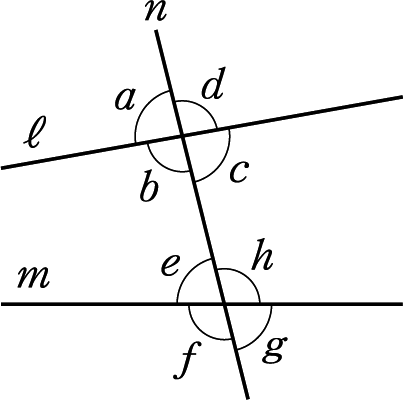
\includegraphics[height=14em,width=16em]{image43.png}

\end{center}
\end{multicols}

(\text{\refstepcounter{skaunta}%
\arabic{skaunta}})\hspace{2.5pt}右の図の四角形ABCDと四角形A'B'C'D'は合同で、対応する頂点がAとA'、BとB'、CとC'、DとD'であるとする。このようなとき、
\begin{align*}
\mbox{四角形ABCD} \framebox[1.5cm][c]{\raise 0.2ex\hbox{\textcircled{\scriptsize{エ}}}} \mbox{四角形A'B'C'D'}
\end{align*}
と表す。


\vfill
\noindent\fbox{\large\makebox[1em]{\text{\refstepcounter{kaunta}%
\arabic{kaunta}}}} \hspace{1pt}三角形の合同条件を3つ書きなさい。

%
\begin{flushright}%
\footnotesize{<知・技$2\times 3$点>}%
\end{flushright}%


\setcounter{skaunta}{0}

\vfill

\noindent\fbox{\large\makebox[1em]{\text{\refstepcounter{kaunta}%
\arabic{kaunta}}}} \hspace{1pt}次の問に答えなさい。

%
\begin{flushright}%
\footnotesize{<知・技$4\times 5$点>}%
\end{flushright}%


(\text{\refstepcounter{skaunta}%
\arabic{skaunta}})\hspace{2.5pt}五角形の外角の和は何度ですか。

\vspace{10mm}

(\text{\refstepcounter{skaunta}%
\arabic{skaunta}})\hspace{2.5pt}十一角形の内角の和は何度ですか。

\vspace{10mm}

(\text{\refstepcounter{skaunta}%
\arabic{skaunta}})\hspace{2.5pt}二十二角形の内角の和は何度ですか。

\vspace{10mm}

(\text{\refstepcounter{skaunta}%
\arabic{skaunta}})\hspace{2.5pt}正十角形の1つの内角の大きさは何度ですか。

\vspace{10mm}

(\text{\refstepcounter{skaunta}%
\arabic{skaunta}})\hspace{2.5pt}正九角形の1つの外角は何度ですか。

\vspace{10mm}

\vfill

\setcounter{skaunta}{0}

\newpage

\noindent\fbox{\large\makebox[1em]{\text{\refstepcounter{kaunta}%
\arabic{kaunta}}}} \hspace{1pt}下の図で、$\angle x$の大きさを求めなさい。ただし、(1)、(2)、(4)では$l /\!/m$とします。

%
\begin{flushright}%
\footnotesize{<知・技(1)$\sim$(5)$4\times 5$点、(6)5点>}%
\end{flushright}%


\begin{multicols}{3}

(\text{\refstepcounter{skaunta}%
\arabic{skaunta}})\hspace{2.5pt}

\begin{tikzpicture}[line cap=round,line join=round,>=triangle 45,x=1.0cm,y=1.0cm,scale=0.8]
\begin{scope}
\clip(-1.32,-3.0) rectangle (3.0,0.7);
\draw [shift={(2.48,-0.32)}] (0,0) -- (41.96060043107308:0.3) arc (41.96060043107308:180.:0.3) -- cycle;
\draw [shift={(0.1,-2.46)}] (0,0) -- (0.:0.4) arc (0.:41.96060043107309:0.4) -- cycle;
\draw (-1.32,-2.46)-- (3.0,-2.46);
\draw [domain=-4.3:17.26] plot(\x,{(-0.96-0.*\x)/3.});
\draw [domain=-4.3:17.26] plot(\x,{(--6.0688-2.14*\x)/-2.38});
\end{scope}
\draw (-1.32,-2.46) node[left] {$m$};
\draw (-1.32,-0.3) node[left] {$l$};
\draw[color=black] (2.3,0.27) node {$x$};
\draw[color=black] (0.96,-2.15) node {$42\textrm{\ensuremath{^\circ}}$};
\end{tikzpicture}

\columnbreak

(\text{\refstepcounter{skaunta}%
\arabic{skaunta}})\hspace{2.5pt}

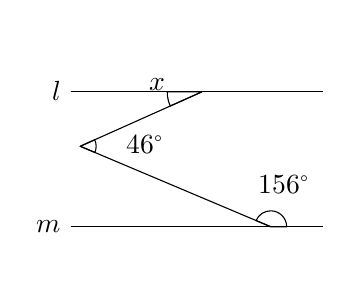
\begin{tikzpicture}[line cap=round,line join=round,>=triangle 45,x=1.0cm,y=1.0cm,scale=0.8]
\begin{scope}
\clip(-1.6,-3.0) rectangle (2.4,0.7);
\draw [shift={(-1.4532025771065582,-1.182716461415865)}] (0,0) -- (-22.894855939768597:0.25274466284575214) arc (-22.894855939768597:24.09272185806487:0.25274466284575214) -- cycle;
\draw [shift={(0.47608168261601636,-0.32)}] (0,0) -- (180.:0.5476134361657963) arc (180.:204.09272185806486:0.5476134361657963) -- cycle;
\draw [shift={(1.5713085549476091,-2.46)}] (0,0) -- (0.:0.25274466284575214) arc (0.:157.10514406023142:0.25274466284575214) -- cycle;
\draw [domain=-3.5931073892005934:5.488850829056767] plot(\x,{(-0.96-0.*\x)/3.});
\draw (0.47608168261601636,-0.32)-- (-1.4532025771065582,-1.182716461415865)-- (1.5713085549476091,-2.46);
\draw [domain=-3.5931073892005934:5.488850829056767] plot(\x,{(-7.38-0.*\x)/3.});
\end{scope}
\draw[color=black] (-0.87,-1.1532295840838602) node[right] {$46\textrm{\ensuremath{^\circ}}$};
\draw[color=black] (-0.23160337335209014,-0.45396935021061385) node[above] {$x$};
\draw[color=black] (1.7819291073190686,-2.10) node[above] {$156\textrm{\ensuremath{^\circ}}$};
\draw (-1.6,-2.46) node[left] {$m$};
\draw (-1.6,-0.3) node[left] {$l$};
\end{tikzpicture}

\columnbreak

(\text{\refstepcounter{skaunta}%
\arabic{skaunta}})\hspace{2.5pt}

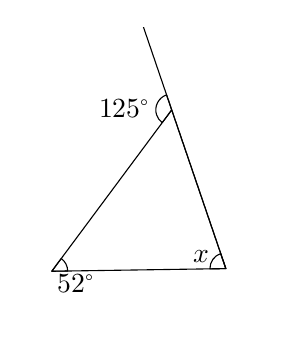
\begin{tikzpicture}[line cap=round,line join=round,>=triangle 45,x=1.0cm,y=1.0cm,scale=0.8]
\begin{scope}
\clip(-1.6,-3.0) rectangle (2.4,1.85);
\draw (0.6867022349874774,0.5443720680301056) -- (-1.217307558450522,-2.016773848806845) -- (1.5460340886630346,-1.974649738332553) -- cycle;
\draw [shift={(0.6867022349874774,0.5443720680301056)}] (0,0) -- (108.83641418112641:0.25274466284575214) arc (108.83641418112641:233.37211054329245:0.25274466284575214) -- cycle;
\draw [shift={(-1.217307558450522,-2.016773848806845)}] (0,0) -- (0.8733436290601997:0.25274466284575214) arc (0.8733436290601997:53.37211054329248:0.25274466284575214) -- cycle;
\draw [shift={(1.5460340886630346,-1.974649738332553)}] (0,0) -- (108.83641418112641:0.25274466284575214) arc (108.83641418112641:180.8733436290602:0.25274466284575214) -- cycle;
\draw [domain=-2.733775535525034:1.5460340886630346] plot(\x,{(-2.1976141627209373--2.519021806362659*\x)/-0.8593318536755572});
\end{scope}
\draw[color=black] (0.5,0.565434123267252) node[left] {$125\textrm{\ensuremath{^\circ}}$};
\draw[color=black] (-0.8297657420870344,-1.9) node[below] {$52\textrm{\ensuremath{^\circ}}$};
\draw[color=black] (1.158492272299549,-1.7850912411982391) node {$x$};
\end{tikzpicture}
\end{multicols}

\begin{multicols}{3}
(\text{\refstepcounter{skaunta}%
\arabic{skaunta}})\hspace{2.5pt}

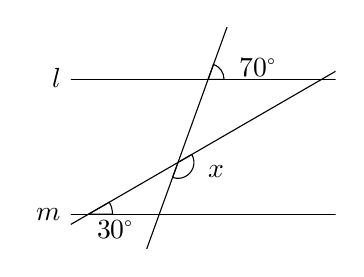
\begin{tikzpicture}[line cap=round,line join=round,>=triangle 45,x=1.0cm,y=1.0cm,scale=0.8]
\begin{scope}
\clip(-1.6,-3.0) rectangle (2.6,0.5);
\draw [shift={(0.5771795477543171,-0.32)}] (0,0) -- (0.:0.25274466284575214) arc (0.:70.09018990725646:0.25274466284575214) -- cycle;
\draw [shift={(0.09944396498145282,-1.6390243013350516)}] (0,0) -- (-109.90981009274356:0.25274466284575214) arc (-109.90981009274356:30.044160069925958:0.25274466284575214) -- cycle;
\draw [shift={(-1.32,-2.46)}] (0,0) -- (0.:0.3791169942686282) arc (0.:30.044160069925976:0.3791169942686282) -- cycle;
\draw [domain=-3.593107389200593:5.0591849022189885] plot(\x,{(-0.96-0.*\x)/3.});
\draw [domain=-3.593107389200593:5.0591849022189885] plot(\x,{(-7.38-0.*\x)/3.});
\draw [domain=-3.593107389200593:5.0591849022189885] plot(\x,{(--1.48319099466687-2.14*\x)/-0.7750836327269732});
\draw [domain=-3.593107389200593:5.0591849022189885] plot(\x,{(-6.2772--2.14*\x)/3.7});
\end{scope}
\draw[color=black] (0.92,-0.13382611060599475) node[right] {$70\textrm{\ensuremath{^\circ}}$};
\draw[color=black] (0.43395757214172426,-1.7850912411982394) node[right] {$x$};
\draw[color=black] (-0.89,-2.4) node[below] {$30\textrm{\ensuremath{^\circ}}$};
\draw (-1.6,-2.46) node[left] {$m$};
\draw (-1.6,-0.3) node[left] {$l$};
\end{tikzpicture}

\columnbreak

(\text{\refstepcounter{skaunta}%
\arabic{skaunta}})\hspace{2.5pt}

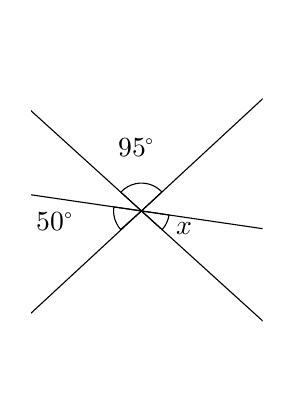
\begin{tikzpicture}[line cap=round,line join=round,>=triangle 45,x=1.0cm,y=1.0cm,scale=1.4]
\begin{scope}
\clip(-1.3,-2.5) rectangle (0.8,0.8);
\draw [shift={(-0.29900195011095404,-0.8625732218112449)}] (0,0) -- (42.78524487268073:0.25274466284575214) arc (42.78524487268073:137.78524487268075:0.25274466284575214) -- cycle;
\draw [shift={(-0.29900195011095404,-0.8625732218112449)}] (0,0) -- (171.6768795548645:0.25274466284575214) arc (171.6768795548645:221.6768795548645:0.25274466284575214) -- cycle;
\draw [shift={(-0.29900195011095404,-0.8625732218112449)}] (0,0) -- (-42.21475512731927:0.25274466284575214) arc (-42.21475512731927:-8.323120445135478:0.25274466284575214) -- cycle;
\draw [domain=-3.652081143864599:5.000211147554982] plot(\x,{(-0.9061493576629651-0.7250381001409278*\x)/0.7991919229402396});
\draw [domain=-3.652081143864599:5.000211147554982] plot(\x,{(--0.46394411162362154-0.73295952225268*\x)/-0.79193327691669});
\draw [domain=-3.652081143864599:5.000211147554982] plot(\x,{(-0.8294487106994136-0.13388852658629502*\x)/0.9151869779762016});
\end{scope}
\draw[color=black] (-0.341126060585246,-0.4623941723054708) node[above] {$95\textrm{\ensuremath{^\circ}}$};
\draw[color=black] (-0.8213409199921751,-0.959458675902116) node[left] {$50\textrm{\ensuremath{^\circ}}$};
\draw[color=black] (0.08853986625253257,-1.0184324305661245) node {$x$};
\end{tikzpicture}

\columnbreak

(\text{\refstepcounter{skaunta}%
\arabic{skaunta}})\hspace{2.5pt}

\begin{tikzpicture}[line cap=round,line join=round,>=triangle 45,x=1.0cm,y=1.0cm,scale=1.5]
\begin{scope}
\clip(-2.6,-2.5) rectangle (1.9672751934059567,0.8);
\draw [shift={(-2.405207473825555,-1.5112845231153405)}] (0,0) -- (0.24381035610408444:0.25274466284575214) arc (0.24381035610408444:32.243810356104085:0.25274466284575214) -- cycle;
\draw [shift={(-0.4253742815338301,-1.502859701020482)}] (0,0) -- (178.47923033885624:0.25274466284575214) arc (178.47923033885624:308.47923033885627:0.25274466284575214) -- cycle;
\draw [shift={(0.16720130598795951,-2.2483838757432935)}] (0,0) -- (102.97750130006334:0.25274466284575214) arc (102.97750130006334:128.97750130006332:0.25274466284575214) -- cycle;
\draw(-0.30759863161230455,-0.18810870123506507) -- (-2.405207473825555,-1.5112845231153405) -- (-0.4253742815338301,-1.502859701020482) -- (0.16720130598795951,-2.2483838757432935) -- cycle;
\draw [shift={(-0.30759863161230455,-0.18810870123506507)}] (0,0) -- (-147.75618964389594:0.25274466284575214) arc (-147.75618964389594:-77.02249869993669:0.25274466284575214) -- cycle;
\draw (-0.30759863161230455,-0.18810870123506507)-- (-2.405207473825555,-1.5112845231153405);
\draw (-2.405207473825555,-1.5112845231153405)-- (-0.4253742815338301,-1.502859701020482);
\draw (-0.4253742815338301,-1.502859701020482)-- (0.16720130598795951,-2.2483838757432935);
\draw (0.16720130598795951,-2.2483838757432935)-- (-0.30759863161230455,-0.18810870123506507);
\end{scope}
\draw[color=black] (-1.983966369082635,-1.5) node[below] {$32\textrm{\ensuremath{^\circ}}$};
\draw[color=black] (-0.694968588569299,-1.869339462146822) node {$130\textrm{\ensuremath{^\circ}}$};
\draw[color=black] (0.25,-2.0883848366131397) node[right] {$26\textrm{\ensuremath{^\circ}}$};
\draw[color=black] (-0.4422239257235469,-0.5634920374437715) node {$x$};
\end{tikzpicture}

\end{multicols}

\setcounter{skaunta}{0}

\vfill

\noindent\fbox{\large\makebox[1em]{\text{\refstepcounter{kaunta}%
\arabic{kaunta}}}} \hspace{1pt}下の図で合同な三角形の組を見つけ、記号$\equiv$を使って表しなさい。

また、そのとき使った合同条件をいいなさい。

%
\begin{flushright}%
\footnotesize{<知・技$4\times 3$点>}%
\end{flushright}%


\begin{center}
\def\@captype{figure}
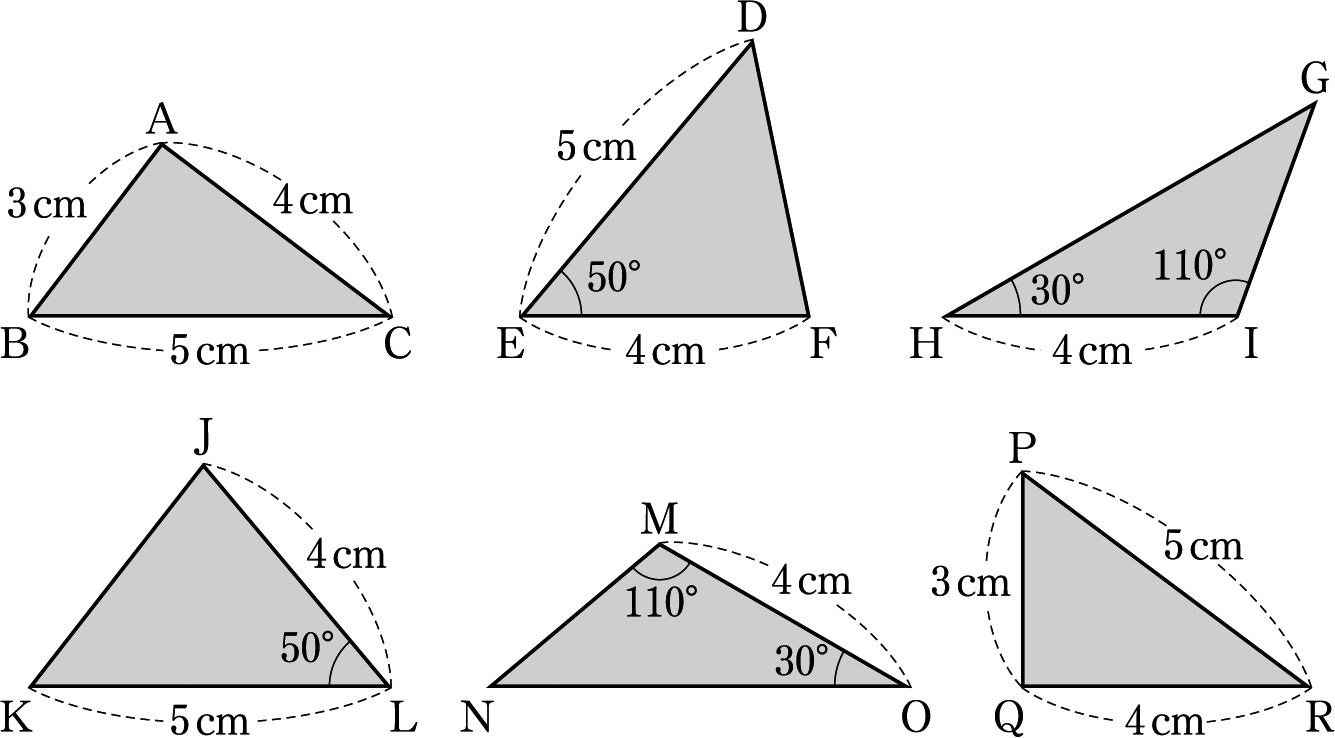
\includegraphics{image71.png}

\vfill
\end{center}

\newpage
\noindent\fbox{\large\makebox[1em]{\text{\refstepcounter{kaunta}%
\arabic{kaunta}}}} \hspace{1pt}下の図で、AE$=$DE、$\angle$BAE $=$ $\angle$CDEならば、AB$=$CDであることを下の図のように証明しました。次の問に答えなさい。

%
\begin{flushright}%
\footnotesize{<知・技(1)4点、思・判・表(2),(3)5点>}%
\end{flushright}%


\begin{multicols}{2}
\begin{screen}
$\triangle$ABEと$\triangle$DCEにおいて
\begin{alignat*}{3}
 \mbox{AE} &= \mbox{DE} \\
 \angle \mbox{BAE} &= \angle \mbox{CDE} \\
 \angle \mbox{AEB} &= \angle \mbox{DEC} \cdots \cdots \mbox{(ア)} \\
 \mbox{したがって} \qquad \triangle \mbox{ABE} &\equiv \triangle \mbox{DCE}\cdots \cdots \mbox{(イ)} \\\\
 \mbox{これより} \qquad \qquad \mbox{AB} &= \mbox{CD}
\end{alignat*}
\end{screen}

\columnbreak

\def\@captype{figure}
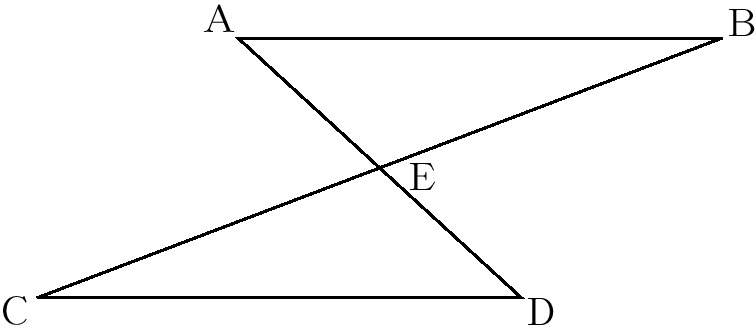
\includegraphics{image7.jpg}

\end{multicols}

(\text{\refstepcounter{skaunta}%
\arabic{skaunta}})\hspace{2.5pt}仮定と結論を書きなさい。

\vspace{15mm}

(\text{\refstepcounter{skaunta}%
\arabic{skaunta}})\hspace{2.5pt}(ア)の根拠となることがらを答えなさい。

\vspace{15mm}

(\text{\refstepcounter{skaunta}%
\arabic{skaunta}})\hspace{2.5pt}(イ)の根拠となる三角形の合同条件を書きなさい。

\vspace{15mm}

\setcounter{skaunta}{0}

\vfill

\newpage

\begin{multicols}{2}
\noindent\fbox{\large\makebox[1em]{\text{\refstepcounter{kaunta}%
\arabic{kaunta}}}} \hspace{1pt}右の図のように、平行な直線$l, \, m$上に等しい長さの線分AB、CDをそれぞれとります。

%
\begin{flushright}%
\footnotesize{<思・判・表(1)10点、(2)5点>}%
\end{flushright}%


\columnbreak

\def\@captype{figure}
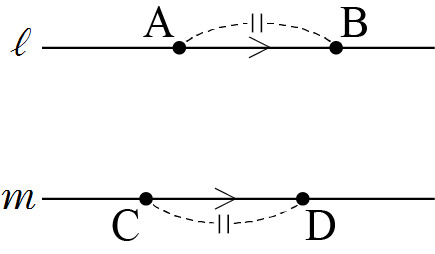
\includegraphics{image15.jpg}

\end{multicols}

(\text{\refstepcounter{skaunta}%
\arabic{skaunta}})\hspace{2.5pt}このとき、AC$=$DBとなることを下の図のように、AとDを結ぶ線分をひいて証明しました。証明を完成しなさい。

\begin{center}
\def\@captype{figure}
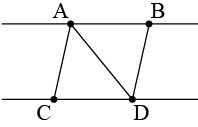
\includegraphics{image23.jpg}

\end{center}

\vspace{15mm}

(\text{\refstepcounter{skaunta}%
\arabic{skaunta}})\hspace{2.5pt}下の図のように、線分ADと線分BCの交点をOとすると、点Oは線分ADと線分BCの中点となることを証明するために、次のような【証明の方針】を立てましたが、証明できませんでした。

【証明の方針】のア、イ、ウだけで三角形の合同が示せるように方針を見直すとき、
見直す部分をアからウの中から1つ選び、記号で答えなさい。また、その部分を見直した内容を書きなさい。

\begin{multicols}{2}

\begin{center}
\def\@captype{figure}
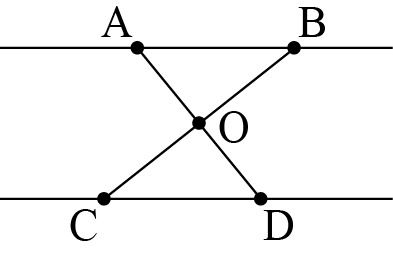
\includegraphics{image37.jpg}

\end{center}

\begin{framed}
結論

「点Oは線分ADと線分BCの中点となる。」

$\rightarrow$ AO $=$ OD、BO $=$ CO
\end{framed}

\columnbreak

【証明の方針】

\begin{framed}
結論を証明するために
$\triangle \mbox{AOB} \equiv \triangle \mbox{DOC}$を示せばよい。

\begin{center}
$\downdownarrows$
\end{center}

$\triangle \mbox{AOB} \equiv \triangle \mbox{DOC}$の辺や角について、次のことがいえそうだ。
\setlength{\abovedisplayskip}{1pt}
\setlength{\belowdisplayskip}{1pt}
\begin{align*}
\mbox{AB} &= \mbox{DC} \cdots \cdots \cdots \mbox{\refstepcounter{kcounter}\ifthenelse{\value{kcounter}=1}{ア}{\ifthenelse{\value{kcounter}=2}{イ}{\ifthenelse{\value{kcounter}=3}{ウ}{\ifthenelse{\value{kcounter}=4}{エ}{\ifthenelse{\value{kcounter}=5}{オ} {\ifthenelse{\value{kcounter}=6}{カ}{\ifthenelse{\value{kcounter}=7}{キ}{\ifthenelse{\value{kcounter}=8}{ク}{\ifthenelse{\value{kcounter}=9}{ケ}{\ifthenelse{\value{kcounter}=10}{コ}{\ifthenelse{\value{kcounter}=11}{サ}{\ifthenelse{\value{kcounter}=12}{シ}{\ifthenelse{\value{kcounter}=13}{ス}{\ifthenelse{\value{kcounter}=14}{セ}{\ifthenelse{\value{kcounter}=15}{ソ}{\ifthenelse{\value{kcounter}=16}{タ}{\ifthenelse{\value{kcounter}=17}{チ}{\ifthenelse{\value{kcounter}=18}{ツ}{\ifthenelse{\value{kcounter}=19}{テ}{\ifthenelse{\value{kcounter}=20}{ト}{\ifthenelse{\value{kcounter}=21}{ナ}{\ifthenelse{\value{kcounter}=22}{二}{\ifthenelse{\value{kcounter}=23}{ヌ}{\ifthenelse{\value{kcounter}=24}{ネ}{\ifthenelse{\value{kcounter}=25}{ノ}{\ifthenelse{\value{kcounter}=26}{ハ}{\ifthenelse{\value{kcounter}=27}{ヒ}{\ifthenelse{\value{kcounter}=28}{フ}{\ifthenelse{\value{kcounter}=29}{ヘ}{\ifthenelse{\value{kcounter}=30}{ホ}{\ifthenelse{\value{kcounter}=31}{マ}{\ifthenelse{\value{kcounter}=32}{ミ}{\ifthenelse{\value{kcounter}=33}{ム}{\ifthenelse{\value{kcounter}=34}{メ}{\ifthenelse{\value{kcounter}=35}{モ}{\ifthenelse{\value{kcounter}=36}{ヤ}{\ifthenelse{\value{kcounter}=37}{ユ}{\ifthenelse{\value{kcounter}=38}{ヨ}{\ifthenelse{\value{kcounter}=39}{ラ}{\ifthenelse{\value{kcounter}=40}{リ}{\ifthenelse{\value{kcounter}=41}{ル}{\ifthenelse{\value{kcounter}=42}{レ}{\ifthenelse{\value{kcounter}=43}{ロ}{\ifthenelse{\value{kcounter}=44}{ワ}{・}}}}}}}}}}}}}}}}}}}}}}}}}}}}}}}}}}}}}}}}}}}}} \\
\angle \mbox{AOB} &= \angle \mbox{DOC} \, \cdots \mbox{\refstepcounter{kcounter}\ifthenelse{\value{kcounter}=1}{ア}{\ifthenelse{\value{kcounter}=2}{イ}{\ifthenelse{\value{kcounter}=3}{ウ}{\ifthenelse{\value{kcounter}=4}{エ}{\ifthenelse{\value{kcounter}=5}{オ} {\ifthenelse{\value{kcounter}=6}{カ}{\ifthenelse{\value{kcounter}=7}{キ}{\ifthenelse{\value{kcounter}=8}{ク}{\ifthenelse{\value{kcounter}=9}{ケ}{\ifthenelse{\value{kcounter}=10}{コ}{\ifthenelse{\value{kcounter}=11}{サ}{\ifthenelse{\value{kcounter}=12}{シ}{\ifthenelse{\value{kcounter}=13}{ス}{\ifthenelse{\value{kcounter}=14}{セ}{\ifthenelse{\value{kcounter}=15}{ソ}{\ifthenelse{\value{kcounter}=16}{タ}{\ifthenelse{\value{kcounter}=17}{チ}{\ifthenelse{\value{kcounter}=18}{ツ}{\ifthenelse{\value{kcounter}=19}{テ}{\ifthenelse{\value{kcounter}=20}{ト}{\ifthenelse{\value{kcounter}=21}{ナ}{\ifthenelse{\value{kcounter}=22}{二}{\ifthenelse{\value{kcounter}=23}{ヌ}{\ifthenelse{\value{kcounter}=24}{ネ}{\ifthenelse{\value{kcounter}=25}{ノ}{\ifthenelse{\value{kcounter}=26}{ハ}{\ifthenelse{\value{kcounter}=27}{ヒ}{\ifthenelse{\value{kcounter}=28}{フ}{\ifthenelse{\value{kcounter}=29}{ヘ}{\ifthenelse{\value{kcounter}=30}{ホ}{\ifthenelse{\value{kcounter}=31}{マ}{\ifthenelse{\value{kcounter}=32}{ミ}{\ifthenelse{\value{kcounter}=33}{ム}{\ifthenelse{\value{kcounter}=34}{メ}{\ifthenelse{\value{kcounter}=35}{モ}{\ifthenelse{\value{kcounter}=36}{ヤ}{\ifthenelse{\value{kcounter}=37}{ユ}{\ifthenelse{\value{kcounter}=38}{ヨ}{\ifthenelse{\value{kcounter}=39}{ラ}{\ifthenelse{\value{kcounter}=40}{リ}{\ifthenelse{\value{kcounter}=41}{ル}{\ifthenelse{\value{kcounter}=42}{レ}{\ifthenelse{\value{kcounter}=43}{ロ}{\ifthenelse{\value{kcounter}=44}{ワ}{・}}}}}}}}}}}}}}}}}}}}}}}}}}}}}}}}}}}}}}}}}}}}} \\
\angle \mbox{OAB} &= \angle \mbox{ODC} \, \cdots \mbox{\refstepcounter{kcounter}\ifthenelse{\value{kcounter}=1}{ア}{\ifthenelse{\value{kcounter}=2}{イ}{\ifthenelse{\value{kcounter}=3}{ウ}{\ifthenelse{\value{kcounter}=4}{エ}{\ifthenelse{\value{kcounter}=5}{オ} {\ifthenelse{\value{kcounter}=6}{カ}{\ifthenelse{\value{kcounter}=7}{キ}{\ifthenelse{\value{kcounter}=8}{ク}{\ifthenelse{\value{kcounter}=9}{ケ}{\ifthenelse{\value{kcounter}=10}{コ}{\ifthenelse{\value{kcounter}=11}{サ}{\ifthenelse{\value{kcounter}=12}{シ}{\ifthenelse{\value{kcounter}=13}{ス}{\ifthenelse{\value{kcounter}=14}{セ}{\ifthenelse{\value{kcounter}=15}{ソ}{\ifthenelse{\value{kcounter}=16}{タ}{\ifthenelse{\value{kcounter}=17}{チ}{\ifthenelse{\value{kcounter}=18}{ツ}{\ifthenelse{\value{kcounter}=19}{テ}{\ifthenelse{\value{kcounter}=20}{ト}{\ifthenelse{\value{kcounter}=21}{ナ}{\ifthenelse{\value{kcounter}=22}{二}{\ifthenelse{\value{kcounter}=23}{ヌ}{\ifthenelse{\value{kcounter}=24}{ネ}{\ifthenelse{\value{kcounter}=25}{ノ}{\ifthenelse{\value{kcounter}=26}{ハ}{\ifthenelse{\value{kcounter}=27}{ヒ}{\ifthenelse{\value{kcounter}=28}{フ}{\ifthenelse{\value{kcounter}=29}{ヘ}{\ifthenelse{\value{kcounter}=30}{ホ}{\ifthenelse{\value{kcounter}=31}{マ}{\ifthenelse{\value{kcounter}=32}{ミ}{\ifthenelse{\value{kcounter}=33}{ム}{\ifthenelse{\value{kcounter}=34}{メ}{\ifthenelse{\value{kcounter}=35}{モ}{\ifthenelse{\value{kcounter}=36}{ヤ}{\ifthenelse{\value{kcounter}=37}{ユ}{\ifthenelse{\value{kcounter}=38}{ヨ}{\ifthenelse{\value{kcounter}=39}{ラ}{\ifthenelse{\value{kcounter}=40}{リ}{\ifthenelse{\value{kcounter}=41}{ル}{\ifthenelse{\value{kcounter}=42}{レ}{\ifthenelse{\value{kcounter}=43}{ロ}{\ifthenelse{\value{kcounter}=44}{ワ}{・}}}}}}}}}}}}}}}}}}}}}}}}}}}}}}}}}}}}}}}}}}}}} \\
\end{align*}

\end{framed}

\end{multicols}

\end{flushleft}

\end{document}
